\documentclass[11pt,a4paper]{article}

\usepackage[polish]{babel}
\usepackage{polski}
\usepackage[utf8]{inputenc}
\usepackage[T1]{fontenc}
\usepackage{graphicx}
\usepackage{color}
\usepackage{placeins}
\usepackage[math]{anttor}
\usepackage{natbib}
\frenchspacing

\newcommand{\todo}[1]{\colorbox{yellow}{#1}}

\begin{document}

\title{Automatyczna klasyfikacja i ekstrakcja tematu krótkich notatek w języku polskim}
\author{Paweł Obrok\\pod kierunkiem dr. Michała Korzyckiego}

\maketitle
\pagebreak

\tableofcontents
\pagebreak

\section{Wstęp}
\section{Podstawy teoretyczne}
\section{Procedura badawcza}
\section{Opis danych}
\section{Wyniki i analiza}

Niniejszy rozdział zawiera porównanie różnych aspektów działania algorytmów LDA
i LSI. Na jego końcu znajdują się wnioski jakie można wyciągnąć z zebranych
danych.

\subsection{Tematy}

Tabele \ref{fig:lsi_topics} i \ref{fig:lda_topics} zawierają niektóre tematy
wygenerowane przez algorytmy LSI i LDA skonfigurowane na 100 tematów (po
dziesięć najbardziej znaczących słów w każdym temacie). Pojedynczy wiersz
tabeli zawiera jeden temat - liczby przy tokenach oznaczają wagi poszczególnych
słów w danym temacie.

Tematy uzyskane przy pomocy LDA wydają się bardziej odpowiadać postrzeganiu
tekstu przez człowieka niż te wygenerowane przez LSI.  Przykładowo temat numer 4 w tabeli
\ref{fig:lsi_topics} można interpretować jako ,,nie pogoda i finanse`` ---
możliwość złożenia dwóch tematów postrzeganych przez człowieka w jeden, ale z
przeciwnymi znakami powoduje powstawanie tego typu kombinacji. Tematy wygenerowane
przez LSI bywają złożeniami dwóch różnych konceptów, jednak zawsze mają ten sam znak,
jak na przykład temat numer 5 w tabeli \ref{fig:lda_topics}, który wydaje się łączyć
koncepty ,,muzeum`` i ,,przestępstwo``.

\begin{table}[h]
\label{fig:lsi_topics}
\caption{Tematy wyekstrahowane przez algorytm LSI}
\begin{tabular}{|c|p{\linewidth}|}
\hline
Lp. & Temat \\\hline
1 & 0.269*" + 0.181*- + 0.171*być + 0.161*procent + 0.144*polski + 0.138*rok + 0.119*) + 0.118*złoty + 0.111*( + 0.102*a \\\hline
2 & -0.304*procent + -0.265*wzróść + -0.254*punkt + -0.211*WIG + -0.192*wynieść + -0.191*spaść + -0.180*złoty + -0.165*spółka + -0.158*akcja + 0.158*" \\\hline
3 & 0.482*RATIO + 0.265*mecz + 0.234*: + 0.187*pokonać + 0.182*mistrzostwo + 0.149*) + 0.149*turniej + -0.142*" + 0.119*piłkarski + 0.117*wygrać \\\hline
4 & -0.301*stopień + -0.250*temperatura + -0.240*maksymalny + -0.228*wiatr + -0.222*umiarkowany + -0.216*deszcz + -0.212*słaby + -0.208*opad + -0.181*południe + 0.164*złoty \\\hline
5 & -0.390*złoty + -0.305*grosz + -0.262*dolar + -0.246*euro + 0.210*punkt + -0.195*osiągać + -0.170*milion + 0.159*WIG + -0.147*umocnić + 0.142*procent \\\hline
6 & -0.355*spółka + -0.301*Akcyjna + 0.259*grosz + -0.223*milion + 0.215*zamknięcie + 0.185*euro + 0.180*osiągać + 0.170*punkt + 0.153*dolar + -0.148*bank \\\hline
7 & -0.435*procent + 0.300*spółka + -0.232*rok + 0.212*akcja + -0.191*proca + 0.190*Akcyjna + 0.148*giełda + -0.133*milion + 0.127*zmienić + 0.124*kurs \\\hline
8 & -0.227*RATIO + 0.192*sąd + -0.147*: + 0.147*( + -0.135*unia + -0.129*mecz + 0.127*policja + -0.125*spółka + 0.122*tysiąc + -0.122*AWS \\\hline
9 & 0.313*( + 0.274*) + -0.258*RATIO + -0.165*mecz + -0.158*sąd + -0.144*: + 0.133*wyścig + 0.126*mistrzostwo + 0.120*spółka + 0.120*świat \\\hline
10 & -0.230*sąd + 0.220*europejski + -0.187*AWS + 0.154*unia + -0.148*procent + 0.143*UE + -0.119*wyborczy + -0.118*okręgowy + 0.114*polski + 0.111*milion \\\hline
\end{tabular}
\end{table}

\begin{table}[h]
\label{fig:lda_topics}
\caption{Tematy wyekstrahowane przez algorytm LDA}
\begin{tabular}{|c|p{\linewidth}|}
\hline
Lp. & Temat \\\hline
1 & 0.027*open + 0.026*powodzianin + 0.021*podlaski + 0.018*Słowenia + 0.017*cukrownia + 0.017*najstarszy + 0.013*przedstawiony + 0.012*urodziny + 0.012*rata + 0.012*zrezygnować\\\hline
2 & 0.021*europejski + 0.021*unia + 0.018*UE + 0.012*polski + 0.011*kraj + 0.010*" + 0.009*Litwa + 0.009*unijny + 0.008*państwo + 0.008*NATO\\\hline
3 & 0.032*palestyński + 0.031*Izrael + 0.030*izraelski + 0.023*Palestyńczyk + 0.015*Arafat + 0.013*szaron + 0.013*świętokrzyski + 0.012*zawieszenie + 0.012*autonomia + 0.011*arabski\\\hline
4 & 0.024*sąd + 0.015*aresztować + 0.015*podejrzany + 0.014*rejonowy + 0.013*okręgowy + 0.013*śledczy + 0.013*akt + 0.012*Gdynia + 0.012*oskarżenie + 0.012*Radom\\\hline
5 & 0.016*wierzyciel + 0.013*muzeum + 0.013*wystawa + 0.011*zbiór + 0.011*śląski + 0.011*Brazylijczyk + 0.010*łączny + 0.010*zajmujący + 0.009*przestępczy + 0.009*łódzki\\\hline
6 & 0.032*festiwal + 0.022*woj + 0.017*Białystok + 0.017*letni + 0.014*wielkopolski + 0.014*wrzesień + 0.014*kupno + 0.012*ogólnopolski + 0.012*usuwanie + 0.012*impreza\\\hline
7 & 0.019*siatkarz + 0.011*obniżka + 0.009*noc + 0.007*postać + 0.006*Gorzów + 0.006*artystyczny + 0.006*bóg + 0.006*bandyta + 0.005*nieznany + 0.005*ZSRR\\\hline
8 & 0.012*" + 0.011*general + 0.010*motors + 0.008*Jedwabne + 0.008*kardynał + 0.007*film + 0.007*weekend + 0.007*Józef + 0.007*rocznica + 0.006*odbyć\\\hline
9 & 0.017*świat + 0.016*klasa + 0.016*TP + 0.015*metr + 0.015*( + 0.015*) + 0.014*mistrzostwo + 0.014*zająć + 0.013*AZS + 0.013*bieg\\\hline
10 & 0.044*obligacja + 0.021*Artur + 0.018*włosek + 0.017*pomnik + 0.016*politechnika + 0.016*białostocki + 0.016*społeczność + 0.013*wyeliminować + 0.012*skorzystać + 0.011*wyemitować\\\hline
\end{tabular}
\end{table}

\FloatBarrier

\subsection{Czas działania}

\subsection{Metryki z nadzorem}

\subsubsection{Ranking dokumentów}

Wykresy \ref{ranks_stemming_comparison}, \ref{ranks_no_stemming_comparison}
przedstawiają sumę kwadratów ranków dokumentów z wzorca przygotowanego ręcznie
dla danego zapytania w wynikach działania odpowiednio algorytmów LDA i LSI dla
różnej liczby tematów.

\begin{figure}[h]
\caption{Suma kwadratów ranków dokumentów ze wzorca dla testowego zapytania (z wykorzystanie stemmingu)}
\label{ranks_stemming_comparison}
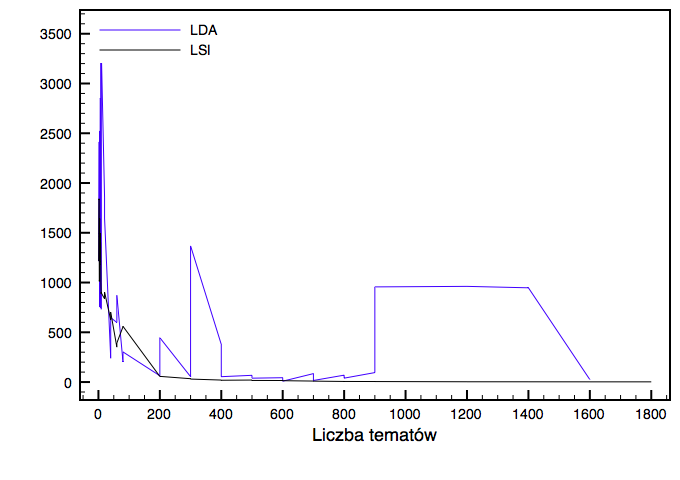
\includegraphics[width=\linewidth]{gfx/ranks_stemming.png}
\end{figure}

\begin{figure}[h]
\caption{Suma kwadratów ranków dokumentów ze wzorca dla testowego zapytania (bez wykorzystania stemmingu)}
\label{ranks_no_stemming_comparison}
\todo{Wykres bez stemmingu}
\end{figure}

\FloatBarrier

\subsection{Krzywe ROC}

Krzywa ROC \cite{roc-article1} (Receiver Operation Characteristic) to wykres przedstawiający dla
danego klasyfikatora stosunek odsetka poprawnie odnalezionych dokumentów wśród
wszystkich dokumentów, które miały zostać odnalezione do odsetka odrzuconych
dokumentów wśród wszystkich dokumentów, które miały zostać odrzucone w miarę
zmiany progu detekcji. W tym wypadku ten zmienny próg to po prostu liczba $n$ -
pierwszych $n$ dokumentów jest traktowane jako odnalezione, a pozostałe jako
odrzucone.

Lepsze klasyfikatory charakteryzują się krzywymi ROC położonymi dalej od linii
$x = y$.  Klasyfikatory blisko, lub na tej linii nie wykonują żadnej użytecznej
pracy. Analiza odległości krzywej ROC od linii $x = y$ w różnych miejscach
wykresu może dać wskazówkę co do najlepszego dobrania progu detekcji dla danego
problemu.

Poniższe wykresy przedstawiają krzywe ROC dla algorytmów LDA i LSI dla różnych
liczb tematów.

\todo{Wykresy bez stemmingu - 20, 100, 300}
\todo{Wykresy ze stemmingiem - 20, 100, 300}

\subsection{Metryki bez nadzoru}

\subsection{Wnioski}

\section{Podsumowanie}

\bibliographystyle{abbrv}
\bibliography{thesis}

\enddocument
